% 第4章第5节：正则性、紧性与边界（嵌入与连续代表、紧嵌入、边界迹、零边界与Poincaré不等式）。

\section{正则性、紧性与边界}
\label{sec:sob-regularity}

Sobolev空间完备，光滑函数在其中稠密，但第~\ref{sec:sob-completeness}节末尾留下的问题还没有回答。本节分别研究四个问题：导数的积分控制能把函数值控制到什么程度；范数有界的函数列能否抽出强收敛子列；体积上的函数怎样拥有边界值；去掉常数方向以后，能否只用导数控制函数本身。四个问题都靠导数控制，但各自需要的条件不同，得到的结论也不能互相替代。

本节除特别说明外，都在有界Lipschitz区域$\Omega\subset\mathbb R^d$上讨论，并且只处理一阶空间$W^{1,p}(\Omega)$。区域有界保证小指数的$L^q$范数受大指数控制（$\|u\|_{L^q}\le|\Omega|^{1/q-1/p}\|u\|_{L^p}$，$q\le p$），边界为Lipschitz保证第~\ref{sec:sob-global-approximation}节的延拓与光滑到边界的逼近可用。

\subsection{积分指数与连续代表}
\label{sec:sob-embedding}

一维时，第~\ref{sec:sob-absolute-continuity}节证明了$W^{1,p}(a,b)$的元素都有连续代表，$p>1$时还是Hölder连续的。可是式~\eqref{eq:sob-power-membership}给出$|x|^{-1/4}\in W^{1,2}(B)$（$B$为$\mathbb R^3$中的单位球），它在原点无界。可见在高维，导数平方可积不足以保证连续。究竟是什么决定了结论？

\paragraph{缩放解释}
设想对全空间上的光滑紧支撑函数$u$有不等式$\|u\|_{L^q(\mathbb R^d)}\le C\|\nabla u\|_{L^p(\mathbb R^d)}$，常数$C$不依赖$u$。把$u$换成$u_\lambda(x)=u(\lambda x)$，$\lambda>0$。由换元$y=\lambda x$，
\[
 \|u_\lambda\|_{L^q}=\lambda^{-d/q}\|u\|_{L^q},\qquad\|\nabla u_\lambda\|_{L^p}=\lambda^{1-d/p}\|\nabla u\|_{L^p} .
\]
不等式对所有$\lambda$成立，两边的$\lambda$指数必须相等，否则令$\lambda\to0$或$\lambda\to\infty$就会破坏它。于是$-d/q=1-d/p$，即
\begin{equation}
 \frac1q=\frac1p-\frac1d,\qquad q=p^*:=\frac{dp}{d-p}\quad(1\le p<d).
 \label{eq:sob-sobolev-exponent}
\end{equation}
称$p^*$为$p$的\term{Sobolev共轭指数}（Sobolev conjugate exponent）。缩放论证只说明了指数必须是什么，并没有证明不等式成立；但它揭示了维数的作用：在$d$维中，把函数压缩到小尺度，导数的$L^p$范数按$\lambda^{1-d/p}$变化，$d$越大、$p$越小，导数就越“看不见”尖锐的集中。当$p>d$时，同样的计算用于Hölder商$|u(x)-u(y)|/|x-y|^\gamma$，它按$\lambda^\gamma$缩放，与$\lambda^{1-d/p}$匹配要求$\gamma=1-d/p$。

\begin{theorem}[Sobolev嵌入]
\label{thm:sob-embedding}
设$\Omega\subset\mathbb R^d$为有界Lipschitz区域。
\begin{enumerate}
 \item 若$1\le p<d$，则$W^{1,p}(\Omega)\subset L^{p^*}(\Omega)$，并存在常数$C$使$\|u\|_{L^{p^*}}\le C\|u\|_{W^{1,p}}$。由区域有界，对$1\le q\le p^*$也有$\|u\|_{L^q}\le C_q\|u\|_{W^{1,p}}$。
 \item 若$d<p<\infty$，则每个$u\in W^{1,p}(\Omega)$有一个在$\overline\Omega$上$\gamma=1-d/p$阶Hölder连续的代表$\tilde u$，并且
 \[
  \sup_{\overline\Omega}|\tilde u|+\sup_{x\neq y}\frac{|\tilde u(x)-\tilde u(y)|}{|x-y|^{\gamma}}\le C\|u\|_{W^{1,p}} .
 \]
\end{enumerate}
\end{theorem}

一个包含关系连同范数控制，称为\term{连续嵌入}（continuous embedding）：包含映射是有界线性算子。图~\ref{fig:sob-embedding-exponents}(a)在$(p,d)$平面上标出两种情形，(b)画出$p^*$随$p$的变化。$H^1=W^{1,2}$在$d=1$时落在Hölder一侧，得到$C^{0,1/2}$，与式~\eqref{eq:sob-1d-holder}一致；$d=3$时落在另一侧，$2^*=6$，得到$L^6$；$d=2$恰好在分界线上。

\begin{figure}[!htb]
  \centering
  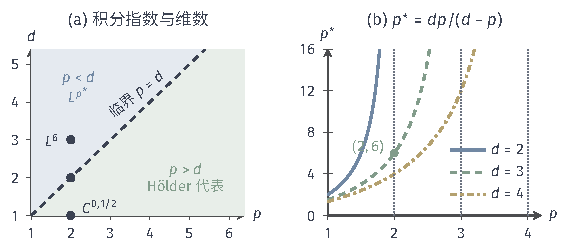
\includegraphics[width=96.3mm]{figures/02-abstract-mathematics/03-function-spaces/tikz/c4-embedding-exponents/figure.pdf}
  \caption{$W^{1,p}$的嵌入由积分指数与维数共同决定。(a)~$(p,d)$平面：$p<d$（蓝）时嵌入$L^{p^*}$，$p>d$（绿）时有Hölder连续代表，虚线$p=d$为临界情形；三个点是$p=2$、$d=1,2,3$，分别得到$C^{0,1/2}$、临界与$L^6$。(b)~$p^*=dp/(d-p)$随$p$增大而增大，$p\to d$时趋于无穷；$d=3$、$p=2$时$p^*=6$。}
  \label{fig:sob-embedding-exponents}
\end{figure}

\paragraph{幂函数检验指数的精确性}
回到$B\subset\mathbb R^d$上的$u=|x|^{-a}$。由式~\eqref{eq:sob-power-membership}，$u\in W^{1,p}(B)$当且仅当$(a+1)p<d$，即$a<d/p-1$；而$u\in L^q(B)$当且仅当$aq<d$。取$q=p^*$，条件$ap^*<d$化为$a<d/p^*=d/p-1$，与前者完全相同。所以每个在$W^{1,p}(B)$中的幂函数都在$L^{p^*}(B)$中，而对任何$q>p^*$，取$a$略小于$d/p-1$，便得到$W^{1,p}(B)$中不属于$L^q(B)$的函数：$p^*$不能再提高。$d=3$、$p=2$时，$a<1/2$的幂函数都在$L^6$中，且无界，这说明$p<d$时一般没有连续代表。

\paragraph{两种结论的机制}
两种情形的证明都从光滑函数出发，再借定理~\ref{thm:sob-smooth-up-to-boundary}推广。$p<d$的情形，先对$\mathbb R^d$上的光滑紧支撑函数证明$\|u\|_{L^{d/(d-1)}}\le\|\nabla u\|_{L^1}$：沿每个坐标方向，$|u(x)|\le\int_{\mathbb R}|\partial_ju|\,\mathrm dx_j$，把$d$个这样的估计相乘开$d-1$次根，再逐个坐标积分并反复使用Hölder不等式。一般的$p$由对$|u|^s$（适当的$s>1$）使用这一估计得到；有界Lipschitz区域上再用延拓算子转移到全空间。这一证明较长，属于补充阅读。

$p>d$的情形可以看出Hölder指数从哪里来。对光滑函数和以$x$为中心、半径$r$的球$B_r$，把$u(x)-u(y)$写成沿线段的导数积分，再对$y\in B_r$取平均，可以得到
\[
 \Bigl|u(x)-\frac{1}{|B_r|}\int_{B_r}u\,\mathrm dy\Bigr|\le C\int_{B_r}\frac{|\nabla u(y)|}{|x-y|^{d-1}}\,\mathrm dy .
\]
右端用Hölder不等式拆成$\|\nabla u\|_{L^p}$与$\bigl(\int_{B_r}|x-y|^{-(d-1)q}\mathrm dy\bigr)^{1/q}$，$q$为共轭指数。后一积分有限当且仅当$(d-1)q<d$，即$p>d$，此时它等于常数乘$r^{1-d/p}$。于是函数值与它在半径$r$的球上的平均之差不超过$Cr^{1-d/p}\|\nabla u\|_{L^p}$；两个相距$r$的点都和同一个球的平均比较，就得到$\gamma=1-d/p$阶的Hölder估计。$p\le d$时核$|x-y|^{1-d}$的$q$次幂不可积，这一步失效。两种结论的区别正在这里：$p<d$时得到的是更高的可积性，由体积上的积分累计；$p>d$时得到的是逐点的振荡控制，靠的是局部平均与中心值的比较。更高的可积性不等于连续，$L^{p^*}$中的函数仍可以无界。

\paragraph{临界情形$p=d$}
$d\ge2$、$p=d$时，两种结论都差一点。一方面，对每个有限的$q$，$W^{1,d}(\Omega)\subset L^q(\Omega)$：区域有界时$W^{1,d}(\Omega)\subset W^{1,s}(\Omega)$对每个$s<d$成立，而$s\to d$时$s^*=ds/(d-s)\to\infty$，所以任意有限$q$都被某个$s^*$超过。另一方面，$W^{1,d}$中的函数一般无界。在单位球$B\subset\mathbb R^d$中取
\[
 u(x)=\ln\ln\frac{e}{|x|} .
\]
记$r=|x|$，$s=\ln(e/r)\ge1$，则$|\nabla u|=1/(rs)$。按球坐标，$\int_B|\nabla u|^d\,\mathrm dx$与$\int_0^1\frac{r^{d-1}}{r^ds^d}\,\mathrm dr=\int_0^1\frac{\mathrm dr}{r\,(\ln(e/r))^d}$成正比，换元$s=\ln(e/r)$后化为$\int_1^\infty s^{-d}\,\mathrm ds$，$d\ge2$时有限；$u$本身只以$\ln\ln$的速度增长，属于$L^d(B)$。所以$u\in W^{1,d}(B)$，却在原点趋于无穷。

一维的$p=1=d$不受这一否定结论影响：第~\ref{sec:sob-absolute-continuity}节已经证明$W^{1,1}(a,b)$的元素有绝对连续代表，当然有界。原因是一维时单点的“容量”不为零：从$x$到$y$只有一条路径，函数的变化必须全部经过它，而在高维中，函数可以绕开一个点集中增长。

\paragraph{高阶空间}
同样的指数比较可以推广到$W^{k,p}$：每多一阶导数，在缩放中多出一个因子$\lambda$。若$kp<d$，则$W^{k,p}(\Omega)\subset L^q(\Omega)$，$1/q=1/p-k/d$；若$kp>d$，则函数有连续代表。特别地，$H^k(\Omega)$的元素在$k>d/2$时有连续代表，并且$\sup|\tilde u|\le C\|u\|_{H^k}$。这一结论使每个点值读取$u\mapsto\tilde u(x)$都是$H^k$上的有界线性泛函，第~\ref{chap:rkhs}章将以此为例说明哪些Hilbert函数空间具有连续的点值。分数阶空间与临界情形的完整分类这里不展开。

\subsection{有界函数列的紧性}
\label{sec:sob-compactness}

第~\ref{sec:sob-completeness}节的例子$u_n=\sin(n\pi x)/(n\pi)$在$H^1(0,1)$中有界，不在$H^1$中收敛，却在$L^2$中收敛。这不是巧合：导数的统一控制阻止了函数在小尺度上剧烈振荡，从而在较弱的范数下迫使序列聚集。

\begin{theorem}[紧嵌入]
\label{thm:sob-rellich}
设$\Omega\subset\mathbb R^d$为有界Lipschitz区域，$1\le p<\infty$。则$W^{1,p}(\Omega)$中的每个有界序列都有一个在$L^p(\Omega)$中收敛的子列。更一般地，$1\le p<d$时可以把$L^p$换成$L^q$，$1\le q<p^*$；$p\ge d$时可以换成任意有限$q$的$L^q$。
\end{theorem}

称这样的包含为\term{紧嵌入}（compact embedding）：包含映射把有界集映成相对紧集，按第~\ref{sec:ose-compact-def}节的说法，它是紧算子。下面给出$L^p$情形的证明，其中用到的延拓定理只给出了证明思路；$L^q$情形的推广由插值不等式得到，从略。

\begin{proof}
设$\|u_n\|_{W^{1,p}(\Omega)}\le M$。只需证明集合$\mathcal F=\{u_n\}$在$L^p(\Omega)$中全有界（第~\ref{sec:metric-totally-bounded}节）：$L^p$完备，完备空间中全有界集的闭包是紧的（定理~\ref{thm:metric-compact-complete-tb}），紧集中的序列有收敛子列。

第一步，转移到全空间。用定理~\ref{thm:sob-extension}的延拓算子，令$w_n=Eu_n$，则$\|w_n\|_{W^{1,p}(\mathbb R^d)}\le\|E\|M=:M'$，且所有$w_n$支撑在同一个有界集合内。只需证明$\{w_n\}$在$L^p(\mathbb R^d)$中全有界，限制到$\Omega$上不增大距离。

第二步，统一的平移估计。对光滑紧支撑函数$w$，$w(x+z)-w(x)=\int_0^1\nabla w(x+tz)\cdot z\,\mathrm dt$，两边取$L^p$范数并把范数移进对$t$的积分（Minkowski积分不等式），得
\[
 \|w(\cdot+z)-w\|_{L^p}\le|z|\,\|\nabla w\|_{L^p} .
\]
两边对$W^{1,p}$范数连续，由定理~\ref{thm:sob-local-approximation}的逼近，它对每个$w\in W^{1,p}(\mathbb R^d)$成立。结合式~\eqref{eq:sob-mollifier-translation}，
\[
 \|w_n*\rho_\varepsilon-w_n\|_{L^p}\le\varepsilon M'\qquad\text{对所有 }n\text{ 一致成立}.
\]
这一步是关键：导数的统一界把所有函数的磨光误差统一控制住了。

第三步，固定$\varepsilon$后的有限网。固定$\varepsilon$，函数$w_n*\rho_\varepsilon$都支撑在同一个紧集$K$内，并且由Hölder不等式，
\[
 |w_n*\rho_\varepsilon(x)|\le\|\rho_\varepsilon\|_{L^q}M',\qquad|\nabla(w_n*\rho_\varepsilon)(x)|\le\|\nabla\rho_\varepsilon\|_{L^q}M' ,
\]
$q$为共轭指数。所以这族函数在$K$上一致有界并有统一的Lipschitz常数。在$K$上取一个间距为$h$的有限网格，每个函数由它在网格点上的值确定到$\|\nabla\rho_\varepsilon\|_{L^q}M'\sqrt d\,h$以内；网格点上的值落在一个有界区间内，把这个区间分成有限多段，就把整族函数分成有限多组，每组内函数的一致距离任意小。一致距离乘$|K|^{1/p}$控制$L^p$距离，所以$\{w_n*\rho_\varepsilon\}$在$L^p$中全有界。这一论证正是第~\ref{sec:apx-arzela-ascoli}节Arzelà--Ascoli定理的机制。

第四步，合并。任给$\eta>0$，先取$\varepsilon$使$\varepsilon M'<\eta/3$，再取$\{w_n*\rho_\varepsilon\}$的有限$\eta/3$网$\{g_1,\ldots,g_N\}$。对每个$n$，选$g_i$与$w_n*\rho_\varepsilon$相距小于$\eta/3$，则$\|w_n-g_i\|_{L^p}<\varepsilon M'+\eta/3<\eta$。所以$\{w_n\}$有有限$\eta$网，全有界。
\end{proof}

证明清楚地显示了三种条件各自的职责。导数的统一界给出统一的平移估计，使磨光误差与$n$无关；区域有界（经延拓后支撑在同一有界集内）使固定尺度的函数族只需有限个网格点描述；目标范数$L^p$比$W^{1,p}$弱，才允许用磨光后的函数近似原函数。

\paragraph{与弱收敛子列的对照}
$1<p<\infty$时，$W^{1,p}(\Omega)$是自反空间，由第~\ref{sec:lfo-weak-subsequence}节，有界序列有弱收敛子列$u_{n_k}\rightharpoonup u$。紧嵌入把这一结论加强了：同一子列在$L^p$中\emph{强}收敛到$u$。原因是紧算子把弱收敛序列映成强收敛序列。在优化与变分问题中，这一组合经常这样使用：从极小化序列的有界性抽出弱收敛子列，再借紧嵌入让低阶项强收敛。但紧嵌入本身只是关于函数列的结论，并不是某个具体方程的可解性定理；把它用于具体问题时，还需要说明目标函数或方程项怎样在这种收敛下保持。

\paragraph{临界指数处的失紧}
定理~\ref{thm:sob-rellich}中$q<p^*$是严格不等式。在临界指数$q=p^*$处，嵌入仍连续，但不再是紧的。取$\varphi\in C_c^\infty(B)$非零，$B$为单位球，$1\le p<d$，令
\[
 u_\lambda(x)=\lambda^{(d-p)/p}\varphi(\lambda x),\qquad\lambda\ge1 .
\]
$u_\lambda$支撑在半径$1/\lambda$的球内。由缩放公式，$\|\nabla u_\lambda\|_{L^p}=\|\nabla\varphi\|_{L^p}$与$\|u_\lambda\|_{L^{p^*}}=\|\varphi\|_{L^{p^*}}$都不随$\lambda$改变，而$\|u_\lambda\|_{L^p}=\lambda^{-1}\|\varphi\|_{L^p}\to0$。所以$(u_\lambda)$在$W^{1,p}(B)$中有界。若某个子列在$L^{p^*}(B)$中收敛，由于它在$L^p$中收敛到$0$，$L^{p^*}$极限也只能是$0$（$L^{p^*}$收敛推出$L^p$收敛），与$\|u_\lambda\|_{L^{p^*}}$恒为常数矛盾。函数的质量向一点集中，在$L^{p^*}$中“看起来”一直一样大，却不收敛到任何东西。图~\ref{fig:sob-compactness-loss}(a)画出$d=3$、$p=2$时的径向剖面$u_\lambda(r)=\lambda^{1/2}\psi(\lambda r)$。

\begin{figure}[!htb]
  \centering
  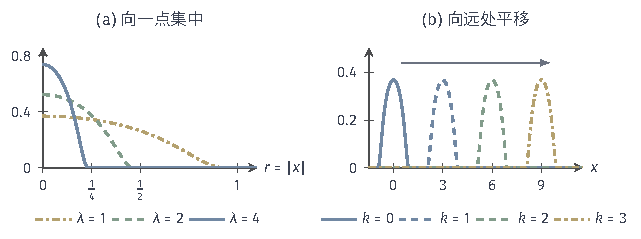
\includegraphics[width=108.6mm]{figures/02-abstract-mathematics/03-function-spaces/tikz/c4-compactness-loss/figure.pdf}
  \caption{两种失去紧性的方式。(a)~临界集中：$d=3$、$p=2$，$u_\lambda(x)=\lambda^{1/2}\psi(\lambda|x|)$的径向剖面，$\lambda=1,2,4$；峰值按$\lambda^{1/2}$升高，支撑半径按$1/\lambda$缩小，$\|\nabla u_\lambda\|_{L^2}$与$\|u_\lambda\|_{L^6}$不变，$\|u_\lambda\|_{L^2}\to0$。(b)~无界区域上的平移：$\psi(x-3k)$，$k=0,1,2,3$，形状和范数都不变，支撑互不相交，向远处逃逸。}
  \label{fig:sob-compactness-loss}
\end{figure}

\paragraph{无界区域上的逃逸}
区域有界的条件也不能去掉。在$\mathbb R^d$上取非零$\varphi\in C_c^\infty(\mathbb R^d)$与单位向量$e$，令$u_n(x)=\varphi(x-3n\,r_0e)$，其中$r_0$使$\operatorname{supp}\varphi\subset B(0,r_0)$。每个$u_n$的$W^{1,p}$范数都等于$\varphi$的范数，支撑两两不交，所以$\|u_n-u_m\|_{L^p}=2^{1/p}\|\varphi\|_{L^p}$（$n\neq m$），任何子列都不是$L^p$中的Cauchy列。函数没有集中，而是整体跑到了无穷远（图~\ref{fig:sob-compactness-loss}(b)，一维时取$\varphi=\psi$、$r_0=1$）。有界区域上，延拓后支撑被限制在同一有界集内，这种逃逸不会发生。

\subsection{边界迹}
\label{sec:sob-trace}

许多问题要给函数指定边界值。可是$W^{1,p}(\Omega)$的元素是几乎处处等价类，而$\partial\Omega$在$\mathbb R^d$中是Lebesgue零测集，任意修改一个代表在边界上的值，得到的仍是同一个元素。“$u$在边界上的值”因此需要重新定义，而不能取一个代表直接限制。

\paragraph{一维端点估计}
一维的答案已经有了。$u\in H^1(a,b)$有唯一的连续代表，式~\eqref{eq:sob-1d-sup-bound}在端点给出
\[
 |\tilde u(a)|\le L^{-1/2}\|u\|_{L^2}+L^{1/2}\|u'\|_{L^2}\le C\|u\|_{H^1(a,b)} .
\]
端点值由$H^1$范数控制，这正是高维要推广的东西。只有$L^2$控制是不够的：$u_n(x)=\max(1-nx,0)$在$(0,1)$上满足$u_n(0)=1$，而$\|u_n\|_{L^2}^2=\int_0^{1/n}(1-nx)^2\,\mathrm dx=1/(3n)\to0$，端点值不受$L^2$范数控制。

\paragraph{半空间上的迹估计}
高维的关键估计可以在半空间上完整证明。设$u\in C_c^\infty(\mathbb R^d)$，限制在$\overline{\mathbb R^d_+}$上考虑。固定$x'\in\mathbb R^{d-1}$，沿$x_d$方向从边界点$(x',0)$向内积分（图~\ref{fig:sob-trace}(b)）：$|u(x',t)|^2$在$t$大时为零，所以
\[
 \begin{aligned}
 |u(x',0)|^2&=-\int_0^\infty\partial_t\bigl(|u(x',t)|^2\bigr)\,\mathrm dt\\
 &\le2\int_0^\infty|u|\,|\partial_du|\,\mathrm dt\le\int_0^\infty\bigl(|u|^2+|\partial_du|^2\bigr)\,\mathrm dt ,
 \end{aligned}
\]
最后一步用了$2ab\le a^2+b^2$。再对$x'\in\mathbb R^{d-1}$积分，得到
\begin{equation}
 \int_{\mathbb R^{d-1}}|u(x',0)|^2\,\mathrm dx'\le\|u\|_{L^2(\mathbb R^d_+)}^2+\|\partial_du\|_{L^2(\mathbb R^d_+)}^2\le\|u\|_{H^1(\mathbb R^d_+)}^2 .
 \label{eq:sob-half-space-trace}
\end{equation}
边界值的$L^2$大小被体积上函数和法向导数的$L^2$大小控制。这与一维端点估计是同一个机制：沿着垂直于边界的每一条线，都是一个一维问题。

\begin{figure}[!htb]
  \centering
  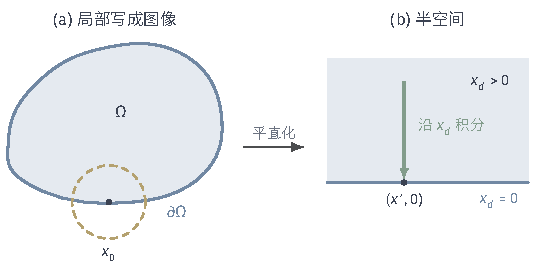
\includegraphics[width=90.3mm]{figures/02-abstract-mathematics/03-function-spaces/tikz/c4-trace/figure.pdf}
  \caption{边界迹的局部化与平直化。(a)~有界Lipschitz区域$\Omega$：边界点$x_0$附近的球（虚线）内，边界是Lipschitz函数的图像，区域位于图像一侧。(b)~拉直后成为半空间$\{x_d>0\}$：从边界点$(x',0)$沿$x_d$方向向内积分，边界值的平方被这条线上$|u|^2+|\partial_du|^2$的积分控制，再对$x'$积分即得式~\eqref{eq:sob-half-space-trace}。}
  \label{fig:sob-trace}
\end{figure}

\paragraph{Lipschitz区域上的迹定理}
在一般的有界Lipschitz区域上，边界需要配上\term{表面测度}（surface measure）$\mathrm dS$。在定义~\ref{def:sob-lipschitz-domain}的一个局部图像$x_d=\gamma(x')$上，约定$\mathrm dS=\sqrt{1+|\nabla\gamma(x')|^2}\,\mathrm dx'$；Lipschitz函数几乎处处可微且梯度有界，所以这个因子在$1$与$\sqrt{1+\mathrm{Lip}(\gamma)^2}$之间，边界上的$L^2$范数与拉直后$\mathbb R^{d-1}$上的$L^2$范数相差有界倍数。不同局部图像重叠处给出相同的测度，这里不加证明地使用这一点。记$L^2(\partial\Omega)=L^2(\partial\Omega,\mathrm dS)$。

\begin{theorem}[迹定理]
\label{thm:sob-trace}
设$\Omega$为有界Lipschitz区域。存在常数$C$，使所有$u\in C^\infty(\overline\Omega)$满足
\begin{equation}
 \|u|_{\partial\Omega}\|_{L^2(\partial\Omega)}\le C\|u\|_{H^1(\Omega)} ,
 \label{eq:sob-trace-inequality}
\end{equation}
并且存在唯一的有界线性算子$\operatorname{Tr}:H^1(\Omega)\to L^2(\partial\Omega)$，对$u\in C^\infty(\overline\Omega)$有$\operatorname{Tr}u=u|_{\partial\Omega}$。
\end{theorem}

式~\eqref{eq:sob-trace-inequality}的证明思路是：用有限个边界球和一个内部开集覆盖$\overline\Omega$，取从属的单位分解，把$u$分成有限块；内部那块在边界上为零；每个边界块用$(x',x_d)\mapsto(x',x_d-\gamma(x'))$拉直，变成半空间上的光滑紧支撑函数，套用式~\eqref{eq:sob-half-space-trace}，再把拉直变换和表面测度因子带来的有界倍数计入常数。这一路线把一维的端点估计逐线推广到一般区域，细节属于补充阅读。

算子$\operatorname{Tr}$的构造则完全可以在这里完成。对$u\in H^1(\Omega)$，由定理~\ref{thm:sob-smooth-up-to-boundary}取$u_n\in C^\infty(\overline\Omega)$在$H^1$中收敛到$u$。由式~\eqref{eq:sob-trace-inequality}，
\[
 \|u_n|_{\partial\Omega}-u_m|_{\partial\Omega}\|_{L^2(\partial\Omega)}\le C\|u_n-u_m\|_{H^1(\Omega)},
\]
所以边界限制构成$L^2(\partial\Omega)$中的Cauchy列，由$L^2$的完备性收敛到某个$g$。极限不依赖逼近列的选取：若$v_n\to u$是另一列，交错排列的$(u_1,v_1,u_2,v_2,\ldots)$仍在$H^1$中收敛到$u$，其边界限制也收敛，于是两个子列的极限相同。令$\operatorname{Tr}u=g$。线性由极限的线性得到，范数界$\|\operatorname{Tr}u\|_{L^2(\partial\Omega)}\le C\|u\|_{H^1(\Omega)}$由式~\eqref{eq:sob-trace-inequality}取极限得到。唯一性来自$C^\infty(\overline\Omega)$的稠密性：两个有界线性算子在稠密子集上一致，便处处一致。

称$\operatorname{Tr}u$为$u$的\term{边界迹}（trace）。它的输出是$L^2(\partial\Omega)$中的等价类，不是某一个边界点上的数：在$d\ge2$时，$H^1$函数可以在边界点附近无界（把前面的幂函数例子中心放到边界点上），单点的值没有意义，只有沿边界的$L^2$平均有意义。迹的像也不是整个$L^2(\partial\Omega)$：可以证明它是一个由边界上“半阶导数”刻画的更小的空间，精确描述需要分数阶Sobolev空间，本章不展开。

\subsection{零边界、零均值与导数控制}
\label{sec:sob-poincare}

有了迹，就可以说一个$H^1$函数“在边界上为零”。本小节用它定义零边界空间，并回答第~\ref{sec:sob-norms}节留下的问题：排除常数方向以后，导数能否单独控制函数。

\paragraph{零边界空间}
第~\ref{sec:sob-global-approximation}节看到，$C_c^\infty(\Omega)$的$H^1$闭包比$H^1(\Omega)$小，它保留了“在边界附近为零”的信息。我们把这个闭包取作定义。

\begin{definition}[零边界Sobolev空间]
\label{def:sob-h01}
设$\Omega\subset\mathbb R^d$为开集。称$C_c^\infty(\Omega)$在$H^1(\Omega)$范数下的闭包为$H_0^1(\Omega)$。
\end{definition}

这个定义不涉及任何代表的边界值，对任意开集都有意义；作为$H^1(\Omega)$的闭子空间，它本身是Hilbert空间。在有界Lipschitz区域上，它可以用迹刻画。$C_c^\infty(\Omega)$中的函数在边界附近为零，迹为零；$\operatorname{Tr}$连续，零迹在$H^1$极限下保持，所以$H_0^1(\Omega)\subset\ker\operatorname{Tr}$。反向包含也成立：

\begin{theorem}[零迹刻画]
\label{thm:sob-h01-kernel}
设$\Omega$为有界Lipschitz区域，则$H_0^1(\Omega)=\ker\operatorname{Tr}=\{u\in H^1(\Omega):\operatorname{Tr}u=0\}$。
\end{theorem}

反向包含的证明思路是：对零迹的$u$，在每个局部图像中把$u$沿远离边界的方向推进一小段，再乘以在边界附近为零的截断并磨光；零迹保证截断引起的误差随推进距离趋于零。细节属于补充阅读。一维时这一刻画很直观：$H_0^1(a,b)$恰好由连续代表满足$\tilde u(a)=\tilde u(b)=0$的$H^1$函数组成。

\paragraph{固定边界值的函数集合}
设边界数据$g$是某个$G\in H^1(\Omega)$的迹，$g=\operatorname{Tr}G$。所有迹等于$g$的$H^1$函数组成集合
\[
 \{v\in H^1(\Omega):\operatorname{Tr}v=g\}=G+H_0^1(\Omega).
\]
等式成立是因为$\operatorname{Tr}v=\operatorname{Tr}G$等价于$\operatorname{Tr}(v-G)=0$，再用定理~\ref{thm:sob-h01-kernel}。这个集合是闭仿射子空间，它的“方向”是$H_0^1(\Omega)$：在保持边界值的前提下，允许的扰动恰好是零迹函数。这一结构是边值问题弱形式的出发点，但具体方程、变分条件和法向导数的含义需要额外的正则性和目标函数，属于优化与微分方程的话题，这里只建立允许函数的集合。

\paragraph{去除常数方向}
现在回到导数半范数$\|\nabla u\|_{L^2}$。常数的梯度为零，所以在整个$H^1(\Omega)$上，$\|\nabla u\|_{L^2}$不可能控制$\|u\|_{L^2}$。图~\ref{fig:sob-poincare}(a)就是这个反例。要让导数单独控制函数，必须用某种条件排除常数。零边界和零均值是两种典型的方式。

\begin{figure*}[!htb]
  \centering
  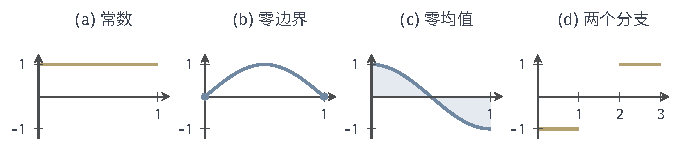
\includegraphics[width=114.4mm]{figures/02-abstract-mathematics/03-function-spaces/tikz/c4-poincare/figure.pdf}
  \caption{Poincaré不等式中约束的作用。(a)~常数$u=1$：$u'=0$而$\|u\|_{L^2}=1$，没有约束时导数控制不了函数。(b)~零边界$u=\sin(\pi x)$：$\|u\|_{L^2}/\|u'\|_{L^2}=1/\pi$。(c)~零均值$u=\cos(\pi x)$（阴影正负面积相等）：比值同为$1/\pi$。(d)~两个分支$(0,1)\cup(2,3)$上分别取$-1$与$1$：均值为零、导数为零，说明零均值形式需要区域连通。}
  \label{fig:sob-poincare}
\end{figure*}

\begin{theorem}[Poincaré不等式]
\label{thm:sob-poincare}
\begin{enumerate}
 \item 设$\Omega$为有界开集。存在常数$C$，使所有$u\in H_0^1(\Omega)$满足$\|u\|_{L^2}\le C\|\nabla u\|_{L^2}$。
 \item 设$\Omega$为有界连通Lipschitz区域，$u_\Omega=|\Omega|^{-1}\int_\Omega u\,\mathrm dx$为均值。存在常数$C$，使所有$u\in H^1(\Omega)$满足$\|u-u_\Omega\|_{L^2}\le C\|\nabla u\|_{L^2}$。
\end{enumerate}
\end{theorem}

\paragraph{区间上的直接证明}
先在区间$(a,b)$上用积分表示直接证明，$L=b-a$。对零边界情形，由$H_0^1$的定义和稠密性，只需对$u\in C_c^\infty(a,b)$证明（两边对$H^1$范数连续）。此时$u(a)=0$，$u(x)=\int_a^xu'(t)\,\mathrm dt$，由Cauchy--Schwarz不等式$|u(x)|^2\le(x-a)\|u'\|_{L^2}^2$，对$x$积分得
\[
 \|u\|_{L^2}^2\le\frac{L^2}{2}\|u'\|_{L^2}^2,\qquad\|u\|_{L^2}\le\frac{L}{\sqrt2}\|u'\|_{L^2} .
\]
对零均值情形，用连续代表，$|\tilde u(x)-\tilde u(y)|\le L^{1/2}\|u'\|_{L^2}$（式~\eqref{eq:sob-1d-holder}，$p=2$）。由于$\tilde u(x)-u_\Omega=L^{-1}\int_a^b(\tilde u(x)-\tilde u(y))\,\mathrm dy$，有$|\tilde u(x)-u_\Omega|\le L^{1/2}\|u'\|_{L^2}$，平方后对$x$积分得$\|u-u_\Omega\|_{L^2}\le L\|u'\|_{L^2}$。这两个常数都不是最优的。在$(0,1)$上，$\sin(\pi x)$与$\cos(\pi x)$分别满足零边界与零均值，比值$\|u\|_{L^2}/\|u'\|_{L^2}$都等于$1/\pi\approx0.318$（图~\ref{fig:sob-poincare}(b)(c)）；可以证明$L/\pi$就是两种情形的最优常数，而上面的直接估计给出$L/\sqrt2\approx0.707L$与$L$。

\paragraph{一般区域的反证路线}
高维没有这样简单的积分表示，但紧嵌入提供了一条反证路线。以零均值情形为例。反设不等式不成立，则对每个$n$有$u_n\in H^1(\Omega)$，$u_n$的均值为零，$\|u_n\|_{L^2}=1$，而$\|\nabla u_n\|_{L^2}<1/n$。

第一步，序列在$H^1$中有界（$\|u_n\|_{H^1}^2<1+1/n^2$），由定理~\ref{thm:sob-rellich}，有子列（仍记作$u_n$）在$L^2$中收敛到某个$u$。$L^2$收敛保持范数与均值，所以$\|u\|_{L^2}=1$，$u$的均值为零。

第二步，极限在$H^1$中取得，且梯度为零。由于$\|u_n-u_m\|_{H^1}^2=\|u_n-u_m\|_{L^2}^2+\|\nabla u_n-\nabla u_m\|_{L^2}^2$，前一项因$L^2$收敛而趋零，后一项不超过$(1/n+1/m)^2$，所以$(u_n)$是$H^1$中的Cauchy列。由定理~\ref{thm:sob-complete}，它在$H^1$中收敛，极限只能是$u$，并且$\|\nabla u\|_{L^2}=\lim\|\nabla u_n\|_{L^2}=0$。

第三步，梯度为零的函数在连通区域上是常数。由式~\eqref{eq:sob-mollifier-commute}，$\nabla(u*\rho_\varepsilon)=(\nabla u)*\rho_\varepsilon=0$在$\Omega_\varepsilon$上成立。对闭包含于$\Omega$的任一球$B$，$\varepsilon$足够小时$B\subset\Omega_\varepsilon$，光滑函数$u*\rho_\varepsilon$在连通的$B$上为常数；令$\varepsilon\to0$，由局部$L^2$恢复，$u$在$B$上几乎处处等于这些常数的极限。相交的两个球上常数相同，而连通开集中任意两点可以用有限个依次相交的球连接，所以$u$在$\Omega$上几乎处处为同一个常数。均值为零迫使这个常数为零，与$\|u\|_{L^2}=1$矛盾。

零边界情形的反证几乎相同。先说明可以只在球上讨论：取一个闭包包含$\overline\Omega$的开球$B_0$，把$H_0^1(\Omega)$的函数在$\Omega$外补成零。对$C_c^\infty(\Omega)$中的函数，零延拓属于$C_c^\infty(B_0)$，$H^1$范数不变；由闭包的定义，零延拓把$H_0^1(\Omega)$等距地映入$H_0^1(B_0)$，并且像中的函数在$B_0\setminus\Omega$上为零。于是只需对球$B_0$上、在$B_0\setminus\Omega$上为零的$H_0^1$函数证明不等式。$B_0$是连通的Lipschitz区域，第一步的紧嵌入可用；第二步的极限$u$仍属于闭子空间$H_0^1(B_0)$，在$B_0\setminus\Omega$上为零，梯度为零；第三步给出$u$在$B_0$上为常数，而$B_0\setminus\Omega$包含一个正测度的环形区域，所以常数为零，同样矛盾。这一论证不需要$\Omega$连通或有Lipschitz边界。

\paragraph{条件为什么不能少}
反证路线清楚地显示了每个条件的作用：紧嵌入把“导数趋于零”变成一个强收敛的极限；弱梯度为零只能推出“在每个连通分支上为常数”；最后由零边界或零均值把常数消去。去掉连通性，零均值不足以消去常数，图~\ref{fig:sob-poincare}(d)在$(0,1)\cup(2,3)$上取$-1$与$1$，均值为零、导数为零，不等式失败。去掉约束，常数函数本身就是反例。去掉区域有界，紧嵌入失效：在整条实轴上，$u_R(x)=\psi(x/R)$满足$\|u_R\|_{L^2}=R^{1/2}\|\psi\|_{L^2}$而$\|u_R'\|_{L^2}=R^{-1/2}\|\psi'\|_{L^2}$，比值随$R$无界，零边界也救不回来。
